\scanpage{116}

CORNU\qquad Ph.\qquad 16/06/78
\mspage{\uline{V}}

C4.Math

\figure{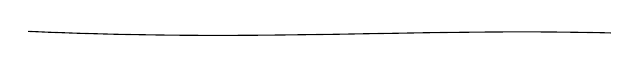
\begin{tikzpicture}[x=1cm,y=1cm]\draw (0,0) .. controls (3,-.13) and (5,.04) .. (7.4,-.02);\end{tikzpicture}}

On peut définir ainsi
\diagram{\begin{tikzcd}[ampersand replacement=\&,row sep=small]
\rho:\quad A\arrow[r]\&A\\
a\arrow[r,maps to]\&\rho(a)
\end{tikzcd}}
avec
\[
a\in C_a\longrightarrow\rho(a)\in\rho'(C_a)
\]

Donc Notons \deleted{\illegible{1}}
\[
\bar A=A/(\underline a)\simeq\mathcal C
\]

$\bar A$ se décompose en 5 ``paquets'' de 3 ``cercles''

On appelle chaque paquet un trièdre, Soit $\mathcal T$ l'ensemble des trièdres.

On a donc l'isomorphisme $\mathcal T\simeq\bar A/(\rho)$

ou $\bar A/(\rho)$ désigne l'ensemble des classes, d'éléments de $\bar A$, modulo $\rho$.

On dira que deux arêtes sont orthogonales si elles sont distinctes et si elles appartiennent à la meme orbite sous $\rho$

\uline{\unsure{ie}}
\[
a_1\perp a_{\unsure{2|1}}
\Longleftrightarrow
a_1=\rho(a_2)\quad\text{ou}\quad a_1=\rho^{-1}(a_2)
\]

On remarque que si deux arêtes sont orthogonales elles n'ont pas de Sommets en Commun

Notons $A(s)$ l'ensemble des arêtes issues de $s$.

On a $A(s)\xrightarrow{\sim}\mathcal T$.

En effet on a $|A(s)|=|\mathcal T|=5$

D'autre part si deux arêtes \deleted{sont} distinctes sont dans $A(s)$, elles ont un sommet en commun, $\uline{s}$, et donc elles n'appartiennent pas au meme trièdre $\Rightarrow$ injectivité

On a bien une bijection

\margin{115}
